\begin{comment}
	%%%%Overview%%%%
	- summary of object class recognition
		- reit challenges from introduction
		- reit of goals - categorisation/localisation
		- one class or multi?
		- show figure 2
			- discuss differences and similarities 
		- general implementation pipeline
	- key challenges - cite robustness/scalability
	- intro to older (non-CNN/deep) methods
		- find from survey
		- eg hand picked feature extractors/SVMS
		- sliding window approaches
		- DPM
	- CNN based methods - taken over since Alexnet (2012) on Imagenet
		- was this classification
		- extended to object detection (use classification network)
		- increase in complexity with CNNs, increase in time per window
			- overcome with region proposals
		- became a 2 step process
			1. find a number of region proposals where an object may be situated
			2. determine if a given proposal is a given pre-defined class
		- overview of proposal methods
			- grouping & window scoring
				- summary of both
			- should be accurate & have high repeatability (see why in dollar cite)
		- pipeline therefore:
			- with a given region proposal method apply deep-based classifier on regions
			- multiple current SOTA do this or similar
				- R-CNN, Fast R-CNN, Faster R-CNN (accurate but not real-time)
				- SSD, YOLOv2/YOLO9000, R-FCN 
					- alternatives to R-CNN 
						- often use some of the same methods (RPN)
				- best instance segmentation COCO 2016 - 2nd best bbox COCO 2016 (2016????)

- important that object detector is translation-invariant
by nature image-level classification favors translation invariance. A shift of an object inside an image should be indiscriminative
However, object detection needs to localise representations that are translation-variant to an extent. Translation of an object inside a candidate box should produce meaningful responses for describing how good candidate box overlaps object
CITE: R-FCN 2016

\end{comment}

This chapter will outline object detection and it's key challenges. This includes aspects within robustness, computational-complexity and scalability. Once completed the key works within object detection will be analysed, both current state-of-the-art and notable older methods.

\section{Object Detection}
As mentioned in \sectionref{intro}, object detection consists of two larger tasks; classification and localisation. Depending on the problem at hand, object detection can be split into two categories. If only a single class is of interest, such as detecting a specific traffic sign, the object detection task is denoted as class-specific detection. Whereas, the more general case when multiple classes are of interest in an image is denoted as multi-class detection \cite{zhang}. Key challenges such as \gls{pascalvoc}, ImageNet, and \gls{mscoco} are of the latter task. This thesis will be within the multi-class detection domain and take these challenges into account when analysing related works in \sectionref{sota} and determining the algorithm to be implemented and evaluated in \sectionref{methodoverview}. An analysis of these key challenges is done in \sectionref{challenges}. The goal of a detector is to output a list of labels from a predefined list of categories indicating which objects are present and where they are located in an image. Object detection has a number of related fields which share to common goal of categories relevant objects. This can be seen in \figref{objfields}. In all four instances the goal is to categorise the two objects person and skateboard, however, the difference lies in the level of localisation precision. In \figref{objcat}, object categorisation aims to only classify the objects in the image without providing any indication as to where the objects are located. Object class detection in \figref{objbb}, localises the classified objects with the use of bounding-boxes, where ideally the bounding-boxes are placed as tightly around the given object as possible. Figure-ground segmentation in \figref{objfig}, indicates localisation with a lasso outline around the objects. Finally, in \figref{objseg}, semantic-segmentation localises objects at a pixel-level classifying each pixel that is related to the given object. 


\add[inline]{correct section refs to above}

\begin{figure}[H]
    \centering
    \begin{subfigure}[b]{0.2\textwidth}
        \center
        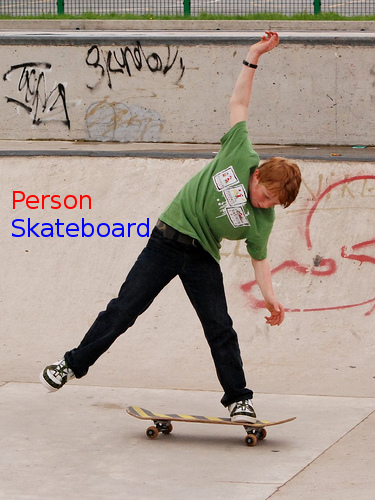
\includegraphics[width=\textwidth]{Figs/Problem/objfieldscat.png}
        \caption{}\label{fig:objcat}
    \end{subfigure}
    \begin{subfigure}[b]{0.2\textwidth}
        \center
        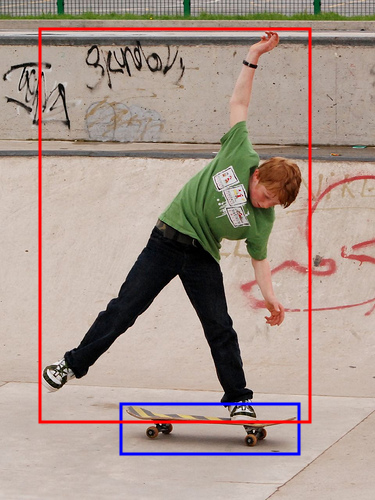
\includegraphics[width=\textwidth]{Figs/Problem/objfieldsbbox.png}
        \caption{}\label{fig:objbb}
    \end{subfigure}
    \begin{subfigure}[b]{0.2\textwidth}
        \center
        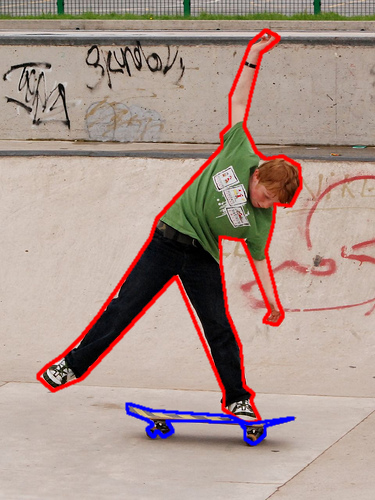
\includegraphics[width=\textwidth]{Figs/Problem/objfieldsfiguresegmentation.png}
        \caption{}\label{fig:objfig}
    \end{subfigure}
    \begin{subfigure}[b]{0.2\textwidth}
        \center
        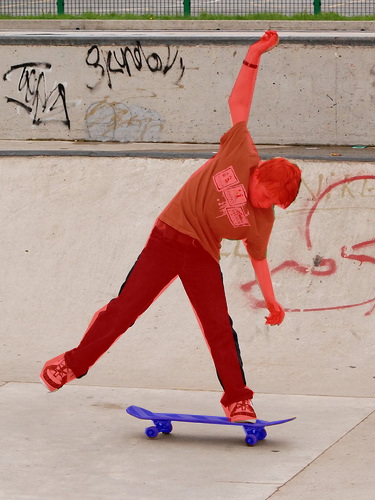
\includegraphics[width=\textwidth]{Figs/Problem/objfieldssegmentation.png}
        \caption{}\label{fig:objseg}
    \end{subfigure}
    \caption{Example of vision tasks related to object detection. All tasks have the common goal of categorising predefined objects. Methods are: object categorisation (a), object class detection (b), figure-ground segmentation (c), semantic Segmentation (d). Image and class labels taken from \gls{mscoco} \cite{mscoco}.}
    \label{fig:objfields}
\end{figure} 

A more recent example of segmentation is that of instance segmentation. Instance segmentation varies to semantic segmentation in that individual instances of objects are classified as such. If multiple instances of the same object is present, such as an image of a crowd with many people, in semantic segmentation all people will be given the same label as one large group. However, in instance segmentation the people are still given the same label but individual instances of a person is also found. This area of research within segmentation is relatively new, however, is beginning to become more popular in comparison to semantic segmentation. For example, the \gls{mscoco} segmentation challenge which has been held in 2015 and 2016 only accepts instance segmentation entries.


\section{Main Challenges}
The challenges of object detection can be split into two groups as per \cite{zhang}:

\begin{itemize}
	\item Robustness-related.
	\item Computational-complexity and scalability-related.
\end{itemize}

Robustness-related refers to the challenges in appearance within the both of intra-class and inter-class. Intra-class is the differences in appearance of objects which are of the same class. For example as seen in \figref{intra_ex}, all of the images belong to the superclass chair from the ImageNet training set \cite{imagenet}, however, vary greatly in their overall appearance. 

\begin{figure}[H]
    \centering
    \begin{subfigure}[b]{0.2\textwidth}
        \center
        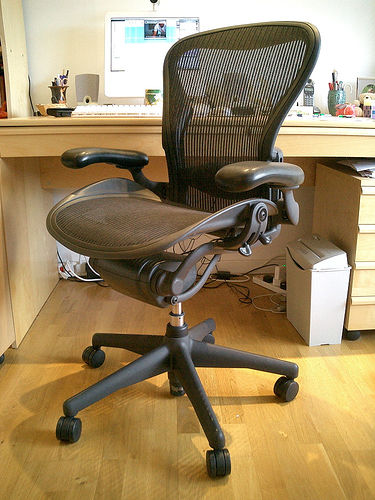
\includegraphics[width=\textwidth]{Figs/Problem/chair1.jpeg}
        \caption{}
    \end{subfigure}
    \begin{subfigure}[b]{0.2\textwidth}
        \center
        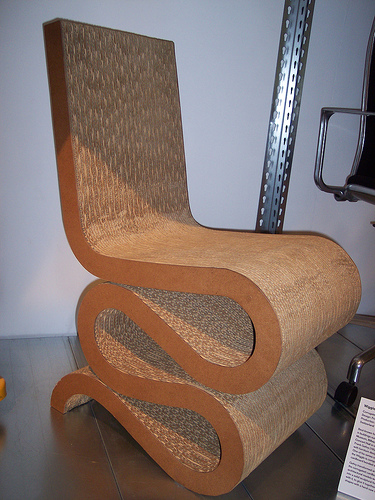
\includegraphics[width=\textwidth]{Figs/Problem/chair2.jpeg}
        \caption{}
    \end{subfigure}
    \begin{subfigure}[b]{0.2\textwidth}
        \center
        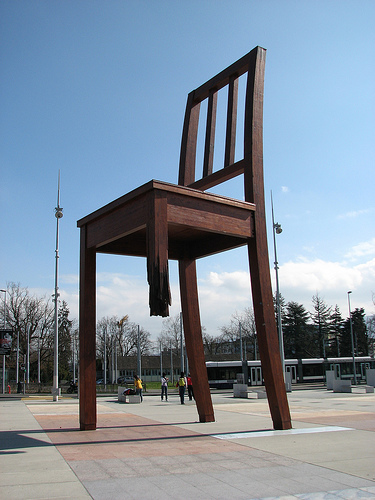
\includegraphics[width=\textwidth]{Figs/Problem/chair3.jpeg}
        \caption{}
    \end{subfigure}
    \begin{subfigure}[b]{0.2\textwidth}
        \center
        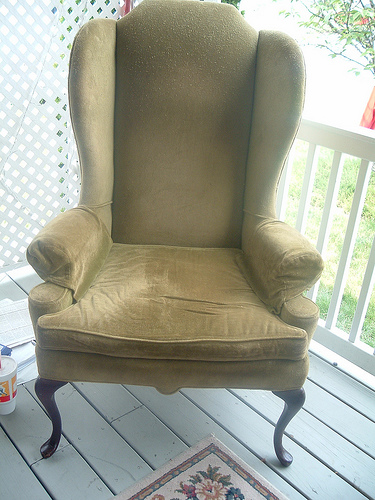
\includegraphics[width=\textwidth]{Figs/Problem/chair4.jpeg}
        \caption{}
    \end{subfigure}
    \caption{Examples of intra-class appearance variation. All images have the label \textit{chair} in the ImageNet training set \cite{imagenet}.}
    \label{fig:intra_ex}
\end{figure} 

An object detection system must be able to learn \add[inline]{explanation that typically obj detection is supervised learning} the appearance variations that can occur intra-class. These variations can be categorised into two types as per \cite{schroff}:

\begin{itemize}
	\item Object variations.
	\item Image variations.
\end{itemize}



\section{Implementation Outline}
As per \cite{zhang} the steps in the general pipeline for an object detection system is as follows:

\begin{enumerate}
	\item Find all possible object regions in the image.
	\item Determine if the regions correspond to any of the predefined categories.
	\item Evaluate all responses from step 2 to determine final detections.
\end{enumerate}


\section{Related Work}